\documentclass[journal,twocolumn]{IEEEtran}
\usepackage{slashbox,graphicx,times,amsmath,amssymb,cite,subfigure,stfloats,booktabs, url,multirow,afterpage}
\usepackage[lined,ruled]{algorithm2e}
\allowdisplaybreaks

\makeatletter
\newcommand{\rmnum}[1]{\romannumeral #1}
\newcommand{\Rmnum}[1]{\expandafter\@slowromancap\romannumeral #1@}
\makeatother


\begin{document}
\title{Motor Imagery for Brain-Computer Interfaces: A Review}

\author{Jingwei~Luo
\thanks{J.~Luo is with the School of Artificial Intelligence and Automation, Huazhong University of Science and Technology, Wuhan, China. Email: d202481524@hust.edu.cn.}}


\markboth{IEEE Transactions on Fuzzy Systems, 2023}%
{Shell \MakeLowercase{\textit{et al.}}: Bare Demo of IEEEtran.cls for IEEE Journals}
\maketitle

\begin{abstract}
% There have been different strategies to improve the performance of a machine learning model, e.g., increasing the depth, width, and/or nonlinearity of the model, and using ensemble learning to aggregate multiple base/weak learners in parallel or in series. This paper proposes a novel strategy called patch learning (PL) for this problem. It consists of three steps: 1) train an initial global model using all training data; 2) identify  from the initial global model the patches which contribute the most to the learning error, and train a (local) patch model for each such patch; and, 3) update the global model using training data that do not fall into any patch. To use a PL model, we first determine if the input falls into any patch. If yes, then the corresponding patch model is used to compute the output. Otherwise, the global model is used. We explain in detail how PL can be implemented using fuzzy systems. Five regression problems on 1D/2D/3D curve fitting, nonlinear system identification, and chaotic time-series prediction, verified its effectiveness. To our knowledge, the PL idea has not appeared in the literature before, and it opens up a promising new line of research in machine learning.
Electroencephalogram-based motor imagery (MI) classification is an important paradigm of non-invasive brain-computer interface (BCI). Among various BCI paradigms, MI has gained significant attention due to its non-invasive nature and potential applications in assistive technology, rehabilitation, and human-computer interaction. This paper provides a comprehensive review of the motor imagery paradigm in BCIs, focusing on its principles, methodologies, and practical applications. We begin by discussing the neural basis of motor imagery and the typical EEG patterns associated with it, such as event-related desynchronization (ERD) and synchronization (ERS). The review then delves into the different experimental setups and signal processing techniques used to detect and classify motor imagery signals, including spatial filtering, feature extraction, and machine learning algorithms. We also examine the challenges and limitations of current MI-based BCIs, such as individual variability, signal noise, and user training requirements. Furthermore, we highlight recent advancements in the field, including hybrid BCI systems, real-time feedback mechanisms, and novel applications in neurorehabilitation and assistive devices. Finally, we discuss future directions and potential research avenues that could enhance the robustness and usability of motor imagery-based BCIs, making them more accessible and effective for a wide range of users.
\end{abstract}

\begin{IEEEkeywords}
Ensemble learning, fuzzy system, patch learning, regression
\end{IEEEkeywords}

\IEEEpeerreviewmaketitle

\section{A BRIEF REVIEW OF EEG-BASED BCI SYSTEMS}

A brain-computer interface (BCI) establishes a direct communication pathway that enables the human brain to interact with external devices \cite{graimann2010brain}. Electroencephalogram (EEG), which records the electrical activities on the scalp of the brain, is the most widely used input signal in non-invasive BCIs due to its affordability and convenience \cite{nicolas2012brain}.

A closed-loop EEG-based BCI system, shown in Fig.~\ref{fig:bci_flowchart}, consists of the following components \cite{wu2020transfer}:
% Machine learning has been widely used in our everyday life, e.g., face recognition \cite{Zhao2003}, natural language processing \cite{Collobert2011}, recommender systems \cite{Wang2015b}, affective computing \cite{drwuVRST2010,drwuMTALR2021}, brain-computer interfaces \cite{drwuiGS2019,drwuEA2020}, etc. However, training a high-performance machine learning model is usually a challenging and iterative process, relying on experience and trial-and-error: a simple model is first designed; if its performance is not satisfactory, then some remedies are taken to enhance it.

% There have been different strategies to enhance the performance of an under-performing machine learning model:
\begin{enumerate}
\item \emph{Signal acquisition} \cite{Liao2012}, which uses an EEG device to collect EEG signals from the scalp. In the early days, EEG devices used wired connections and gel to increase conductivity. Currently, wireless connections and dry electrodes are becoming increasingly popular.

\item \emph{Signal processing} \cite{Makeig2012}, which usually includes temporal filtering and spatial filtering. The former typically uses a bandpass filter to reduce interference and noise, such as muscle artifacts, eye blinks, and DC drift. The latter combines different EEG channels to increase the signal-to-noise ratio. Popular spatial filters include common spatial patterns (CSPs) \cite{ramoser2000optimal}, independent component analysis (ICA) \cite{Makeig1996a}, blind source separation \cite{Jung2000}, xDAWN \cite{rivet2009xdawn}, etc.

\item \emph{Feature extraction}, for which time domain, frequency domain \cite{Wang2014b}, time-frequency domain, Riemannian space \cite{Yger2017}, and/or functional brain connectivity \cite{Wu2019} features could be used.

\item \emph{Pattern recognition}, where depending on the application, a classifier or regression model is used.

\item \emph{Controller}, which outputs a command to control an external device, e.g., a wheelchair or a drone, or to alter the behavior of an environment, e.g., the difficulty level of a video game. A controller may not be needed in certain applications, e.g., BCI spellers.
\end{enumerate}

\begin{figure}[htbp]  % 图片浮动体,h 表示尽可能在此处插入图片
  \centering  % 图片居中
  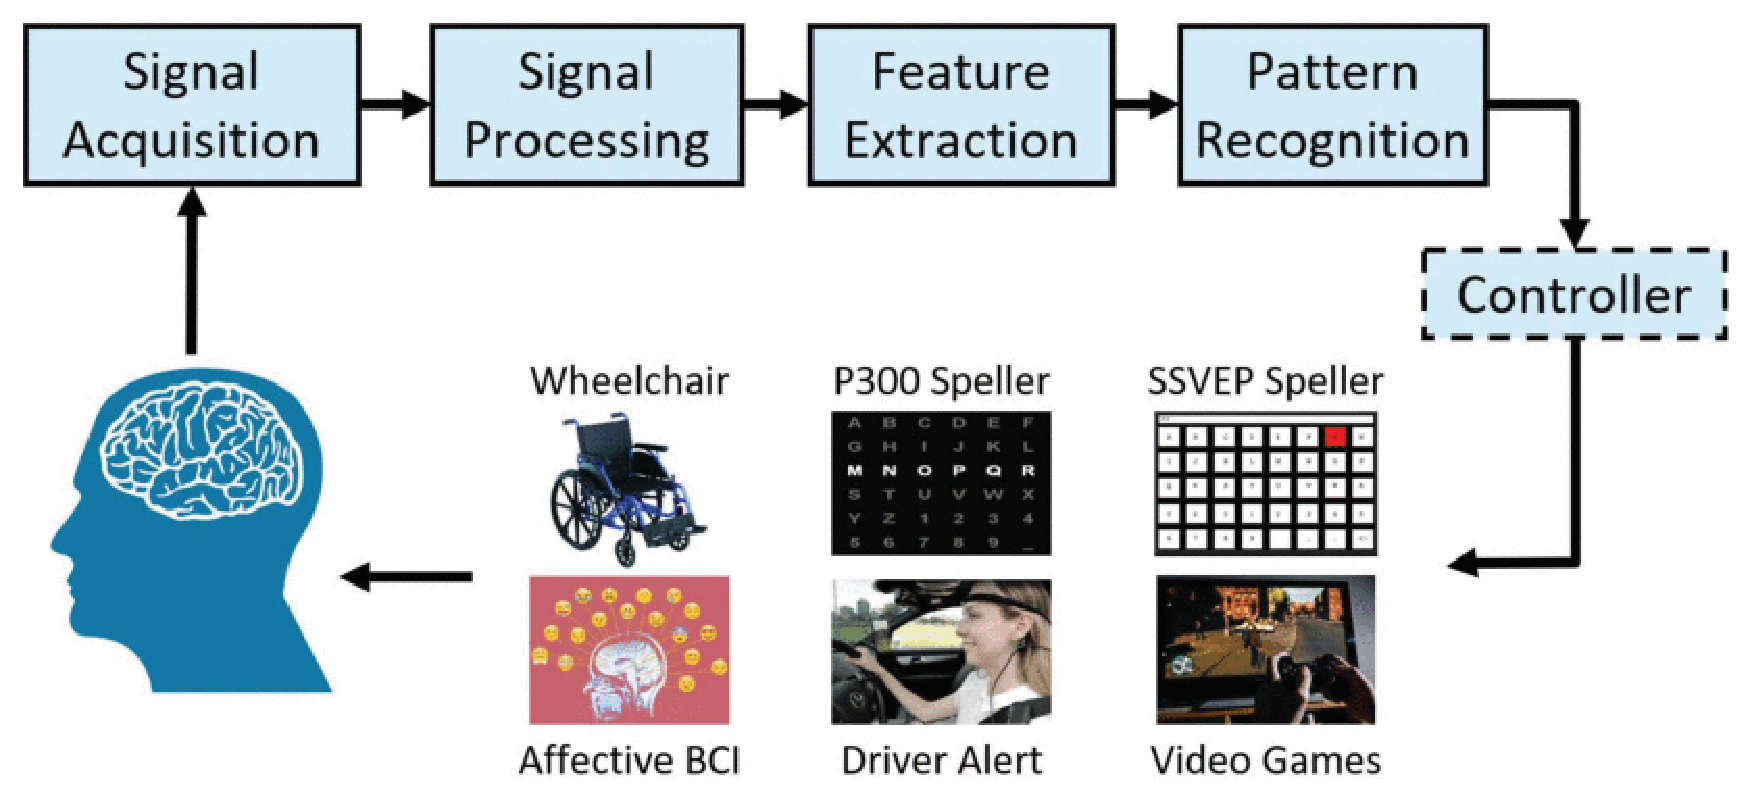
\includegraphics[width=\linewidth]{figures/fig1.eps}  % 插入图片,width 可以设置图片的宽度
  \caption{Flowchart of a closed-loop EEG-based BCI system.}  % 图片标题
  \label{fig:bci_flowchart}  % 给图片设置标签,方便引用
\end{figure}

% \begin{figure}[htbp]\centering
% \subfigure[]{\label{fig:Parallel}   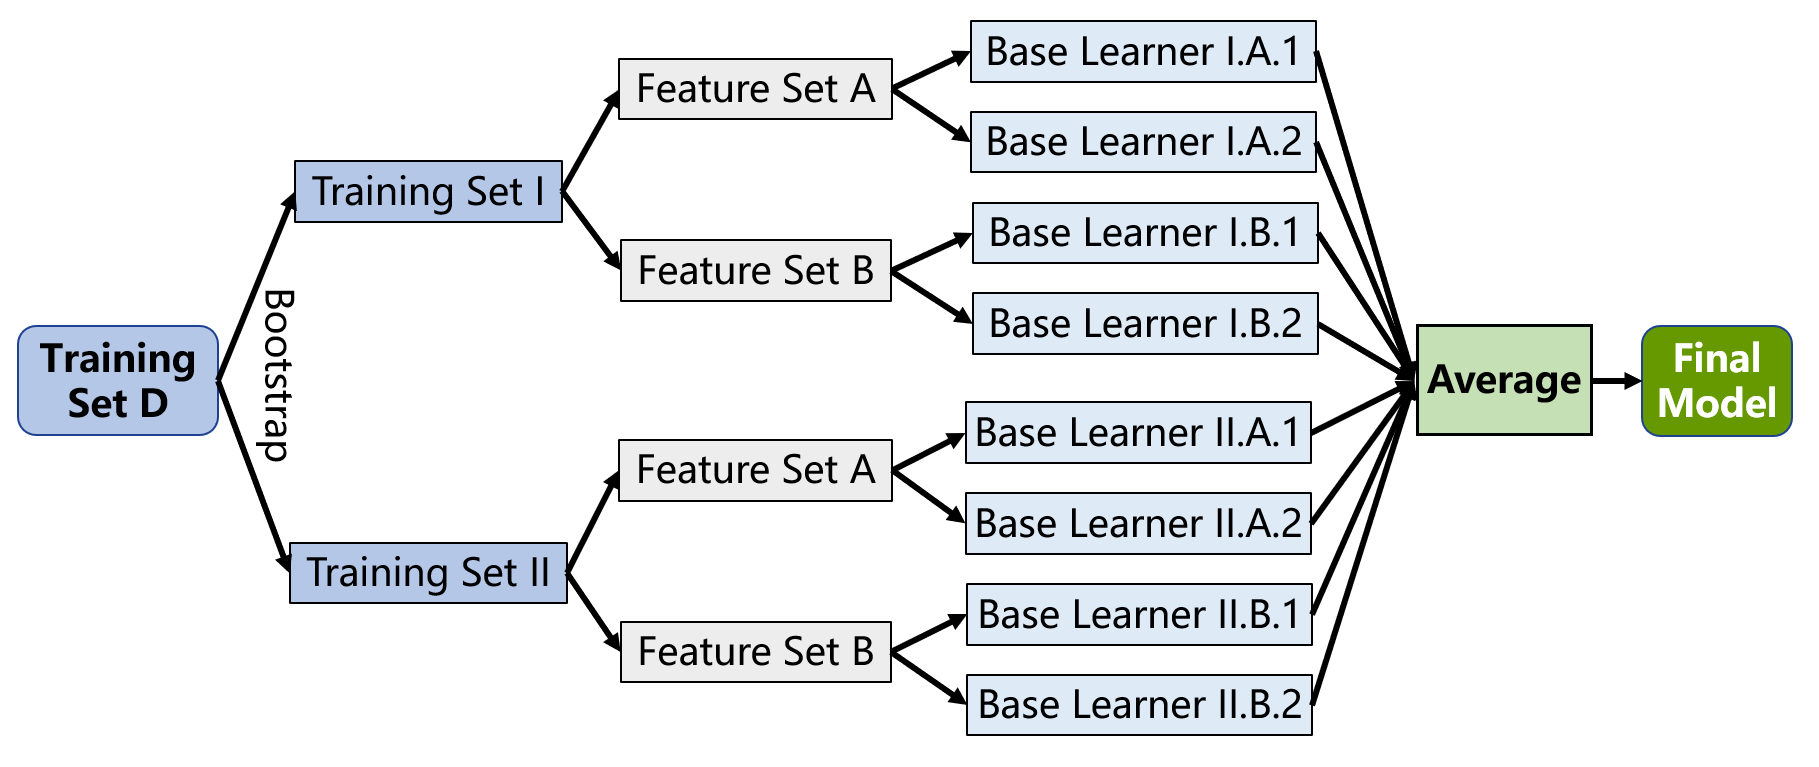
\includegraphics[width=\linewidth,clip]{Fig1a}}
% \subfigure[]{\label{fig:Serial}    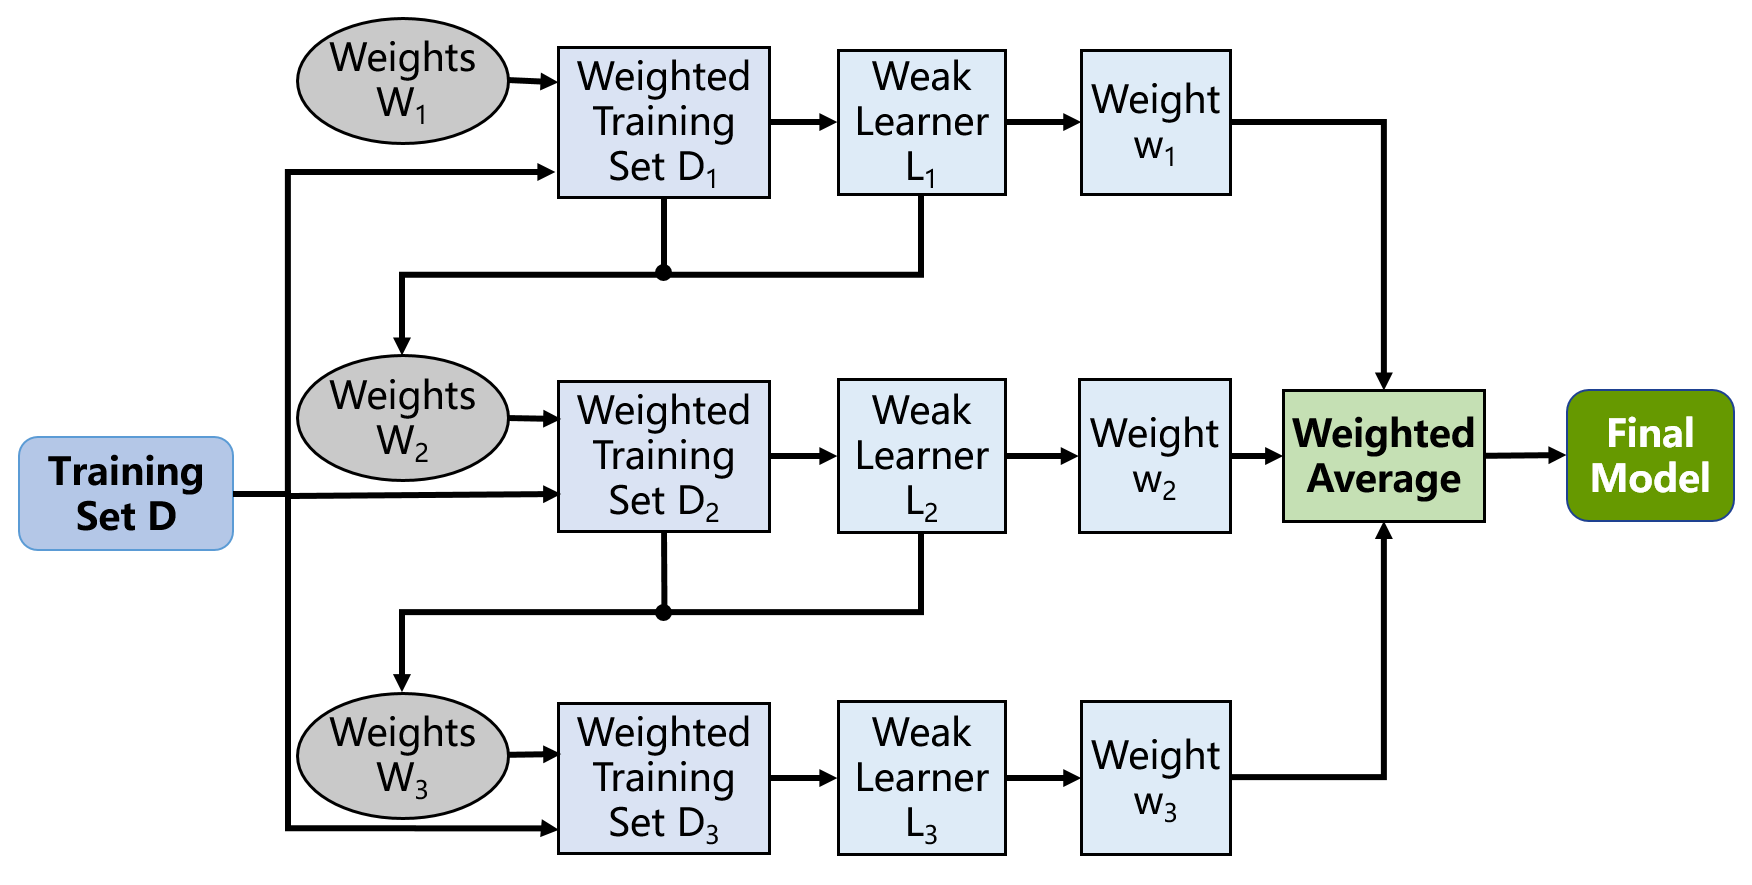
\includegraphics[width=\linewidth,clip]{Fig1b}}
% \subfigure[]{\label{fig:Patch}    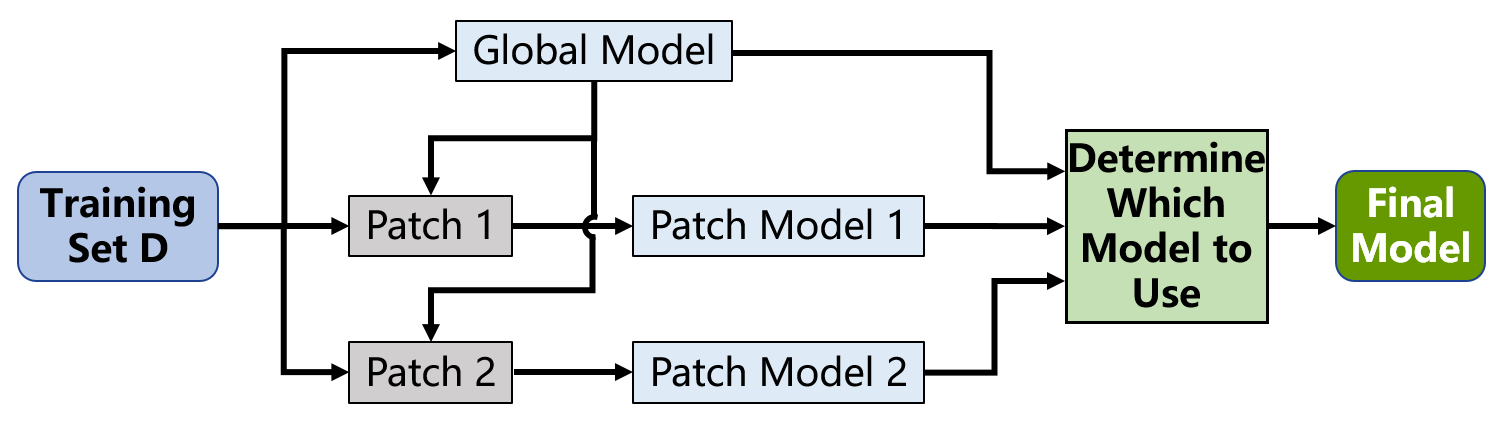
\includegraphics[width=.8\linewidth,clip]{Fig1c}}
% \caption{Strategies for connecting multiple simple models for better performance. (a) parallel ensemble learning; (b) serial ensemble learning (AdaBoost \cite{Freund1997a}); and, (c) PL.} \label{fig:EL}
% \end{figure}

% There are different BCI paradigms, such as steady-state visually evoked potential [3], event-related potential [4], and motor imagery (MI) [5]. This article focuses on MI-based BCIs.

% This paper proposes \emph{patch learning} (PL), which connects multiple simple models both in parallel and in series to improve the learning performance, as illustrated in Fig.~\ref{fig:Patch}. It first trains a global model using all training data, identifies the input regions that give rise to large learning errors, and then designs a patch model for each such region to reduce the overall learning error. The patch models are parallel to and independent of each other, but they are all generated based on the initial global model (and hence in series to the global model). To our knowledge, this idea has not been explored before. We demonstrate the feasibility of PL using fuzzy systems in five regression problems.

% The remainder of this paper is organized as follows: Section~\ref{sect:PL} introduces the general idea of PL, and illustrates it by a simple regression problem. Section~\ref{sect:PLFS} describes in detail how PL can be implemented by fuzzy systems. Section~\ref{sect:experiments} presents five experiments on PL using fuzzy systems to demonstrate its feasibility. Section~\ref{sect:limitations} points out some limitations of the current PL approach, and hence opportunities for future research. Finally, Section~\ref{sect:conclusion} draws conclusions.

\section{Neurophysiological Basis of Motor Imagery} \label{sect:PL}

Motor imagery can be seen as mental rehearsal of a motor act without any overt motor output. This type of phenomenal experience imply that the subject feels himself performing a given action. It corresponds to the so-called internal imagery (or first person perspective) of sport psychologists \cite{landers1983effects}. Motor imagery may be experienced in two ways, or perspectives. The first person perspective which is supposed to rely on motor-kinesthetic information processing, and the third person perspective which would rely more on visuospatial processing. To my knowledge, no neurophysiological or neuroimaging studies concerned with this distinction has been reported. However, a few experiments in cognitive psychology have suggested the relevance to consider the distinction between visual and kinesthetic imagery \cite{denis1985visual}.

Converging evidence from several sources indicates that mental imagination of movements involves similar brain regions/functions which are involved in programming and preparing such movements \cite{jeannerod1995mental}. According to this view, the main difference between performance and imagery is that in the latter case execution would be blocked at some cortico-spinal level \cite{decety1994mapping}.

Functional brain imaging studies monitoring changes in regional cerebral blood flow (rCBF) revealed indeed similar patterns of activity during motor imagery and actual movement performance. An increase of the rCBF has mainly been located in the supplementary motor area during imagination of sequential finger movements \cite{roland1980supplementary}. Moreover, recent positron emission tomography (PET) \cite{decety1994mapping} and functional magnetic resonance imaging (fMRI) studies \cite{rao1993functional} revealed activation of a number of cortical and subcortical areas, including, e.g., the premotor cortex, the anterior cingulate gyrus, superior and inferior parietal areas, and the cerebellum. Thus, activation has been observed in various structures involved in the early stage of motor control (i.e., motor programming), but not in the primary sensorimotor cortex. More recent fMRI studies, in contrast, detected some activation in the primary motor cortex during motor imagery, though to a lesser extent than during actual motor performance \cite{hallett1994involvement}. Increased motor cortex activation during motor imagery has been supported by studies using transcranial magnetic stimulation in showing an increase of motor responses during mental imagination of movements \cite{gandevia1987knowledge}.

Several EEG studies further confirm the notion that motor imagery can activate primary sensorimotor areas \cite{beisteiner1995mental}. It induces changes in the sensory-motor rhythms (SMR) of corresponding areas of the cerebral cortex, which primarily involve modulations of the $\mu$ rhythm (8-12 Hz) and the $\beta$ rhythm (14-30 Hz) \cite{jeannerod1995mental}. Specifically, when an MI starts, these rhythmic activities decrease, resulting in event-related desynchronization (ERD); at the end of an MI, these rhythmic activities increase, resulting in event-related synchronization (ERS) \cite{pfurtscheller1997eeg}.

A blocking of the central mu rhythm with motor imagery was reported in early clinical EEG observations \cite{gastaut1952etude}. Similar cortical activity over the contralateral hand area during execution and imagination of hand movement has further been found with dc potential measurements \cite{beisteiner1995mental} and based on dipole source analysis of electric and magnetic fields \cite{lang1996electric}. Furthermore, high-resolution EEG experiments \cite{pfurtscheller1997motor} showed that independent of the required motor task, imagination versus overt execution of a given movement, the most prominent EEG changes were localized over the corresponding primary sensorimotor cortex. During the imagination of a right-hand or left-hand movement, for example, a similar event-related desynchronization (ERD) over the contralateral hand area as is usually found during planning or preparation of a real movement is found. This imagination-related ERD shows different time courses in the alpha and beta bands (Fig. 2, upper panel). Similar to the self-paced movement task, the ERD in the beta band shows a fast recovery and is followed by a short-lasting event-related synchronization (ERS). Examples for the localization of beta ERS mapped on the reconstructed cortical surface of one representative subject (Fig. 2, lower panel) illustrate a focus close to the primary hand area after both a real executed and an imagined right-hand movement. This observation is in line with recent neuromagnetic studies suggesting that the central 20-Hz activity mainly originates in the primary sensorimotor cortex \cite{salmelin1995functional} and, moreover, documents the supposed similarity of neural circuitry involved in mental representation and movement execution.

It is of interest, that during overt execution of the movement, the initially contralateral ERD develops a bilateral distribution \cite{toro1994event}, whereas during mental simulation this ERD remains mostly limited to the contralateral hemisphere. This means that the suppression of mu and central beta rhythms is more pronounced at the contralateral hemisphere when subjects imagine one-sided hand movements \cite{pfurtscheller1997motor} than when they actually perform such movements. This observation led us to utilize motor imagery as control strategy to achieve asymmetrical electrocortical responses and to use, e.g., left-right differences in the sensorimotor EEG to provide a control option in one dimension \cite{neuper1999enhancement}.
Besides this, MI also applies to different parts of the body such as the movement of the left hand, right hand, tongue \cite{qiao2019deep}, left foot, right foot movement \cite{tariq2020mu}, wrist movement (flexion, extension, pronation, and supination) \cite{ma2019deep}, elbow flexion/extension, forearm pronation/supination, hand open/close \cite{mammone2020deep}, and finger movements \cite{alazrai2019deep}.
% This section introduces the general idea of PL, and illustrates it by a simple example.

% Formally, we define a \emph{patch} as a connected polyhedron in the input domain. For example, a patch in a 1D input domain is an interval, as shown in Fig.~\ref{fig:1Dpatch}, and a patch in a 2D input domain can be a rectangle, an ellipse, etc., as shown in Fig.~\ref{fig:2Dpatch}. For ease of implementation, in this paper we only consider polyhedra whose number of surfaces (sides) equals the dimensionality of the input domain, and each surface (side) is perpendicular to an axis of the input domain, e.g., an interval in the 1D input domain [Patches~1-3 in Fig.~\ref{fig:1Dpatch}], and a rectangle in the 2D input domain [each side is perpendicular to an axis, such as Patch~1 in Fig.~\ref{fig:2Dpatch}].

\begin{figure}[htbp]\centering
\subfigure[]{\label{fig:1Dpatch}   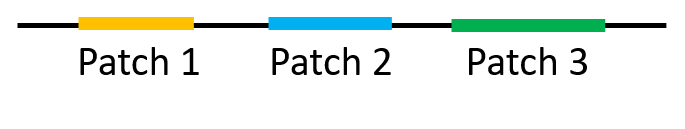
\includegraphics[width=.47\linewidth,clip]{Fig2a}}
\subfigure[]{\label{fig:2Dpatch}    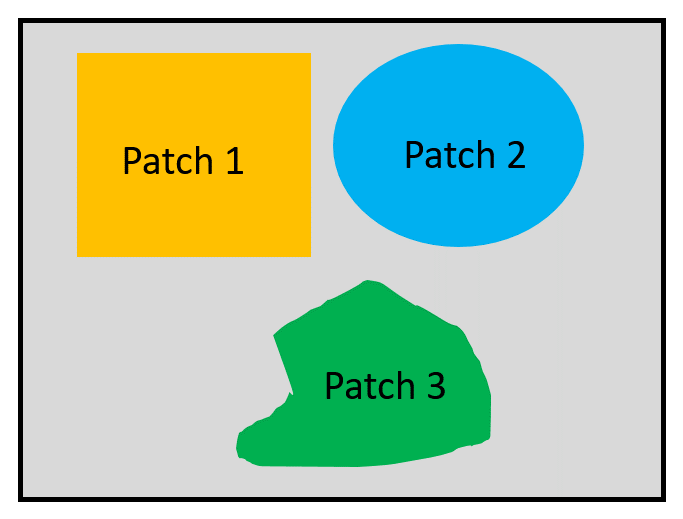
\includegraphics[width=.47\linewidth,clip]{Fig2b}}
\caption{Patches in 1D and 2D input domains.} \label{fig:patchs}
\end{figure}


% \subsection{Steps of PL}

% Given $L$, the number of patch models to be trained, PL consists of the following three steps:
% \begin{enumerate}
% \item Train an initial global model using all training data.
% \item Identify $L$ patches from the initial global model, which contribute the most to the learning error, and train a (local) patch model for each such patch.
% \item Update the global model using training data that do not fall into any patch.
% \end{enumerate}
% The rationale for the last step is that, when the default global model is first trained, it is forced to fit all training examples, some of which, e.g., those within the $L$ patches identified in Step (2), may be really difficult to fit. Since these difficult training examples have been handled by the patch models in Step (2), we can update the default global model to fit only the examples outside of the $L$ patches. This should be much easier than fitting all examples together, and hence the root mean squared error (RMSE) of the default global model may be reduced. Since in Step (3) the training examples for the updated global model are all outside of the patches, the updated global model is not suitable for inputs within any of the $L$ patches: although it can output an arbitrary value for such an input, this does not matter, since the patch models are used to handle such cases.

% The idea of PL may be intuitively understood by making the following analogy. Consider a sculptor who is sculpting a human figure. After his first pass at this, the sculptor examines the entire figure and notices that improvements need to be made to certain parts of the figure. The sculptor does not throw out the entire figure and begin a new. Instead, he zooms into those parts that need more work, after which he blends in the refined portions of the figure with the rest of the figure. He continues such iterative refinements until he is satisfied with the entire figure. Each patch in PL is analogous to a part in the figure that needs more work. In traditional ensemble learning approaches, usually each base/weak learner also focuses on the entire figure, instead of a part of it.

% \subsection{Determine the Optimal Number of Patch Models}

% An important question in PL is how to determine $L$, the optimal number of patch models. Increasing $L$ is equivalent to increasing the model complexity in traditional machine learning. So, some analogy also applies here: generally, the training performance increases with $L$, but the test (generalization) performance may first increase and then decrease (indicating overfitting). Inspired from some common practices in traditional machine learning for reducing overfitting \cite{Duda2000,Hastie2009}, there are at least two approaches to determine $L$ in PL:
% \begin{enumerate}
% \item \emph{Early stopping}. We first partition all available labeled data into a training set and a validation set (these two sets should not overlap). Then, we train different PL models with different $L$ on the training set, and monitor their performances on the validation set. The one with the best validation performance is chosen as the final PL model.
% \item \emph{Regularization}. We view $L$ as an indicator of model complexity, and regularize it in the loss function so that $L$ cannot be too large. We then pick the PL model that results in the smallest loss. There could be different choices and implementations of the regularization, similar to the case in traditional machine learning.
% \end{enumerate}

% The second idea is used in this paper. We mainly consider regression problems, and use the following loss function, which showed satisfactory performance in our experiments:
% \begin{align}
% \ell= rmse(\mathbb{D})\times (L+1)^\alpha, \label{eq:loss}
% \end{align}
% where $rmse(\mathbb{D})$ is the training RMSE on the training set $\mathbb{D}$, and $\alpha>0$ is a trade-off parameter between the RMSE and the model complexity. A smaller $\alpha$ prefers a more accurate but maybe more complex model, and a larger $\alpha$ prefers a simpler model with a smaller number of patches, but the RMSE maybe large. Our experiments showed that $\alpha=1/4$ gave satisfactory performance, so $\alpha=1/4$ was used in this paper.

% \subsection{PL Illustrated by a Simple Example}

% Next, we use a simple regression problem with only one input to illustrate the above procedure.

% \begin{align}
% \theta_s=\arg\min_{\theta_s}\left[\sum_{i=1}^{n_s}(y_{s,i}-x_{s,i})^2+\lambda_1\|\theta_s\|^2\right]
% \end{align}

% Assume we have $N=601$ training examples $(x_n,y_n)$, $n=1,...,N$, generated from the unknown function
% \begin{align}
% y=\left\{\begin{array}{ll}
%            x+x^2+8\sin(x), & x\in[1.5,3] \\
%            x+x^2+2\sin(x), & x\in[4,5] \\
%            x+x^2, & \mbox{otherwise}
%          \end{array}\right. \label{eq:g}
% \end{align}
% where $x\in[0,6]$ and 601 uniform samples are used. The true relationship between $y$ and $x$ is plotted as the dotted black curve in Fig.~\ref{fig:gPL0}. We would like to build a PL model to fit it. The basic nonlinear regression model used is $y=f(x)=\beta_0+\beta_1x+\beta_2x^2$.

% \begin{figure}[htbp]\centering
% \subfigure[]{\label{fig:gPL0}   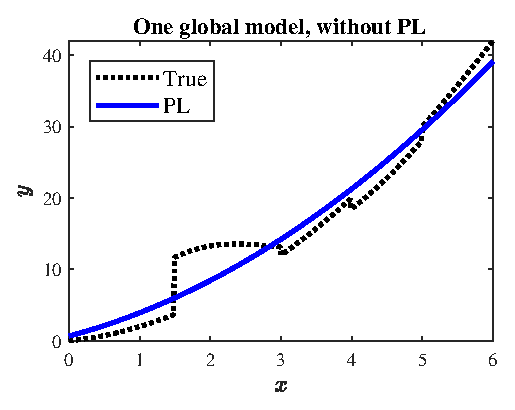
\includegraphics[width=.47\linewidth,clip]{Fig3a}}
% \subfigure[]{\label{fig:gRMSE0}    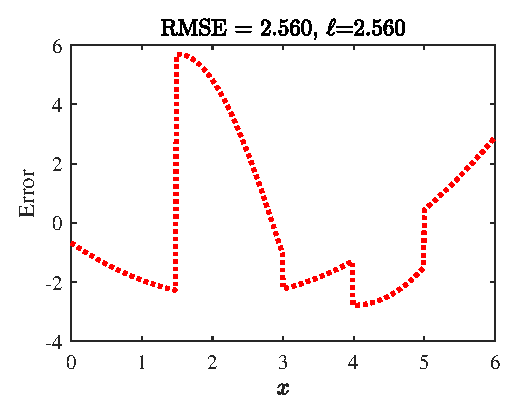
\includegraphics[width=.47\linewidth,clip]{Fig3b}}
% \caption{The general idea of PL, illustrated by a simple 1D curve fitting problem. (a) fitting by one global model $f_g(x)$; (b) the fitting error of $f_g(x)$.} \label{fig:gPL}
% \end{figure}

% The first step is to build a global model $f_g(x)$ using all $N$ training examples. The fitted model is $f_g(x)=0.68+2.63x+0.63x^2$, plotted as the solid blue curve in Fig.~\ref{fig:gPL0}. The fitting errors are shown in Fig.~\ref{fig:gRMSE0}. Clearly, the RMSE is large, i.e., a single global model cannot fit the data well.

% By visual examination of Fig.~\ref{fig:gRMSE0}, we can see that the fitting errors are large when $x\in[1.5,3]$. So, the next step is to build a patch model for $x\in[1.5,3]$. Using only the training examples within this patch, we obtain the first patch model $f_1(x)=1.65+9.81x-2.01x^2$. $f_g(x)$ and $f_1(x)$ together reduce the training RMSE from $2.560$ to $1.654$, and the loss $\ell$ from $2.560$ to $1.967$, as shown in Fig.~\ref{fig:gRMSE1}. The fitting accuracy is improved, but the RMSE may still be too large. So, a second patch model may be needed.

% By visual examination of Fig.~\ref{fig:gRMSE1}, we can see that the fitting errors are large when $x\in[4,5]$. So, the next step is to build a patch model for $x\in[4,5]$. Using only the training examples within this patch, we obtain the second patch model $f_2(x)=19.29-8.03x+1.96x^2$. $f_g(x)$, $f_1(x)$ and $f_2(x)$ together further reduce the training RMSE to $1.332$, and the loss to $1.753$, as shown in Fig.~\ref{fig:gRMSE2}.

% Assume at this point we do not want to add more patches. The final step is then to update the default global model, using all training examples outside of the two patches.  The updated global model is $f'_g(x)=x+x^2$, identical to the last case in (\ref{eq:g}). This step reduces the RMSE to $0.026$, and the loss to $0.035$, as shown in Fig.~\ref{fig:gRMSE3}.

% For the above simple 1D curve fitting example, the final PL model can be easily represented as:
% \begin{align}
% y=\left\{\begin{array}{ll}
%            f_1(x)=1.65+9.81x-2.01x^2, & x\in[1.5,3] \\
%            f_2(x)=19.29-8.03x+1.96x^2, & x\in[4,5] \\
%            f'_g(x)=x+x^2, & \mbox{otherwise}
%          \end{array}\right. \label{eq:g2}
% \end{align}

% Generally, once the PL models are trained, the logic for determining which model to use for a new input is shown in Fig.~\ref{fig:PLmodel}. We first determine if the input falls into any patch. If yes, then the corresponding patch model is used to compute the output. Otherwise, the global model is used.

% \begin{figure}[htbp]         \centering
% 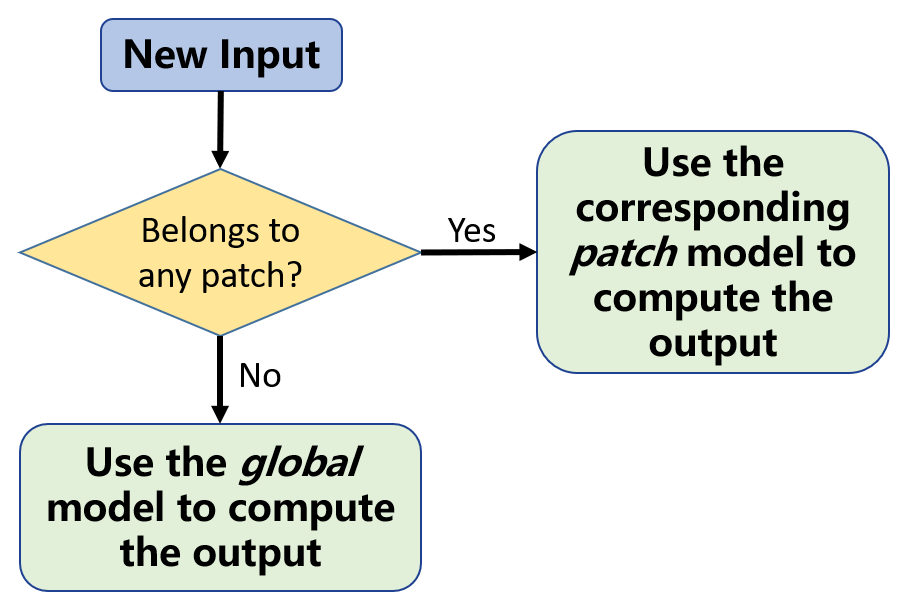
\includegraphics[width=.6\linewidth,clip]{Fig4}
% \caption{The logic for determining which model to use in PL.} \label{fig:PLmodel}
% \end{figure}


% For a well-optimized fuzzy system, transition from one rule partition to another changes the functional form of the input-output mapping. For example,  assume $x_m$ is the only input of the TSK fuzzy system, which has the following three rules:
% \begin{align*}
% R_1: &\mbox{ IF } x_m \mbox{ is } A_1, \mbox{ THEN } y=y_1(x_m)\\
% R_2: &\mbox{ IF } x_m \mbox{ is } A_2, \mbox{ THEN } y=y_2(x_m)\\
% R_3: &\mbox{ IF } x_m \mbox{ is } A_3, \mbox{ THEN } y=y_3(x_m)
% \end{align*}
% where $y_1(x_m)$, $y_2(x_m)$ and $y_3(x_m)$ are different functions of $x_m$. In Partition $P(1|x_m)$, only Rule $R_1$ is fired, and hence the fuzzy system output is $y=f_1(x_m)$; in Partition $P(2|x_m)$, both Rules $R_1$ and $R_2$ are fired, and hence the fuzzy system output is:
% \begin{align}
% y=\frac{\mu_{A_1}(x_m)y_1(x_m)+\mu_{A_2}(x_m)y_2(x_m)}{\mu_{A_1}(x_m)+\mu_{A_2}(x_m)};
% \end{align}
% in Partition $P(3|x_m)$, only Rule $R_2$ is fired, and hence the fuzzy system output is $y=f_2(x_m)$. Clearly, the functional forms of $y$ in the different rule partitions are different. It is reasonable to believe this is because the (unknown) groundtruth functional form changes significantly from one rule partition to another, and hence the fuzzy system uses different functional forms in different rule partitions to accommodate it. Thus, we can consider each such partition as a patch candidate\footnote{This is just one simple way to initialize the patch candidates. There may be better ways to do this.}.

% According to Pedrycz \cite{Pedrycz2018}, \emph{``by information granules one regards a collection of elements drawn together by their closeness (resemblance, proximity, functionality, etc.) articulated in terms of some useful spatial, temporal, or functional relationships. Subsequently, Granular Computing is about representing, constructing, processing, and communicating information granules."} All points within a first-order rule partition fire the same number of same rules, and hence they resemble each other. So, each first-order rule partition can be viewed as an information granule, and PL can be viewed as a form of granular computing.

% \subsection{Implementation Details}

% For the ease of programming implementation, we can use a single index $k\in[1,K]$ to denote a patch candidate (first-order rule partition) $(P(k_1|x_1),P(k_2|x_2),...,P(k_M|x_M))$, where
% \begin{align}
% k&=(k_1-1)\cdot \prod_{m=2}^M K_m+(k_2-1)\cdot \prod_{m=3}^M K_m \nonumber \\
%  &\quad +\cdots+(k_{M-1}-1)\cdot K_M+k_M\nonumber \\
% &=k_M+\sum_{m=1}^{M-1}\left[ (k_m-1)\cdot \prod_{p=m+1}^M K_p\right] \label{eq:k}
% \end{align}
% For example, assume the fuzzy system has two inputs ($M=2$), $x_1$ and $x_2$, each with five first-order rule partitions ($K_1=K_2=5$) shown in Fig.~\ref{fig:Partition}. Then, (\ref{eq:k}) becomes $k=(k_1-1)\times K_2+k_2$. The partition $(P(1|x_1),P(1|x_2))$ is mapped to $k=(1-1)\times 5+1=1$, $(P(1|x_1),P(2|x_2))$ to $k=(1-1)\times 5+2=2$, $\cdots$, $(P(2|x_1),P(1|x_2))$ to $k=(2-1)\times5+1=6$, $\cdots$, and $(P(5|x_1),P(5|x_2))$ to $k=(5-1)\times 5+5=25$.


% For a given $k\in[1,K]$, we can also map it back to a first-order rule partition $(P(k_1|x_1),P(k_2|x_2),...,P(k_M|x_M))$:
% \begin{align}
% k_1&=int\left(\frac{k-1}{\prod_{m=2}^M K_m}\right)+1 \label{eq:k1}\\
% k_2&=int\left(\frac{k-1-(k_1-1)\cdot \prod_{m=2}^M K_m}{\prod_{m=3}^M K_m}\right)+1\\
% k_m&=int\left(\frac{k-1-\sum_{i=1}^{m-1}\left[(k_i-1)\cdot \prod_{p=i+1}^M K_p\right]}{\prod_{p=m+1}^M K_p}\right)+1\\
% k_M&=k-\sum_{m=1}^{M-1}\left[ (k_m-1)\cdot \prod_{p=m+1}^M K_p\right] \label{eq:kM}
% \end{align}
% where $int(x)$ means the integer part of $x$, e.g., $int(2.0)=2$ and $int(2.9)=2$. Using again the above example, when $k=6$, we have $k_1=int(\frac{k-1}{K_2})+1=int(\frac{6-1}{5})+1=2$ and $k_2=k-(k_1-1)\times K_2=6-(2-1)\times 5=1$, and hence the mapped first-order rule partition for $k=6$ is $(P(2|x_1),P(1|x_2))$.

% In summary, the pseudo-code\footnote{A sample Matlab implementation is available at https://github.com/drwuHUST/Patch-Learning.} in Algorithm~\ref{alg:PLFS} implements the three generic PL steps described at the beginning of Section~\ref{sect:PL} using fuzzy systems. Its limitations and potential improvements are discussed in Section~\ref{sect:limitations}, after some experiments to demonstrate its capability are described in the next section.

% \begin{algorithm}[htbp]
% \KwIn{$N$ labeled training examples, $\{(\mathbf{x}_n,y_n)\}^N_{n=1}$, where $\mathbf{x}_n\in\mathbb{R}^{M\times 1}$\;
% \hspace*{9mm} $T$ unlabeled examples, $\{\mathbf{x}_t\}_{t=1}^T$\;}
% \KwOut{The PL model predictions for $\{\mathbf{x}_t\}_{t=1}^T$.}
% \tcp{Train the PL model}
% Train a global fuzzy model using all $N$ training examples\;
% \For{$m=1,...,M$}
% {Identify the first-order rule partitions for the $m$th input domain of the global fuzzy model\;}
% Index the partitions using $k$ in (\ref{eq:k})\;
% Include all partitions in the candidate pool\;
% $l=1$\;
%     \While{$l\le L$}{
%     Identify from the candidate pool the partition giving the maximum SSE\;
%     Record the location of the partition as the $l$th patch\;
%     Train a patch fuzzy model using only the training examples within the $l$th patch\;
%     \If{the $l$th model is successfully trained\footnotemark{}}
%     {$l=l+1$\;}
%     Remove the above patch from the candidate pool\;}
% \caption{PL using fuzzy systems.} \label{alg:PLFS}
% \end{algorithm}



% \begin{table}[h] \centering \setlength{\tabcolsep}{1.5mm}
% \caption{RMSEs, APEs and losses of Bagging and LSBoost in 3D manifold fitting.}   \label{tab:E3}
% \begin{tabular}{c|c|cccccc}   \hline
%  & & \multicolumn{6}{c}{Number of weak learners}\\ \cline{3-8}
% &  & 1 & 2 & 3 &4 &5 & 6\\ \hline
% \multirow{2}{*}{Bagging}&RMSE & 0.2192 &   0.2291 &   0.1546  &  0.1924 & 0.1863 & 0.2337\\
% &APE & 0.0157 &   0.0163 &   0.0111 &   0.0138 & 0.0134 & 0.0168\\ \hline
% \multirow{2}{*}{LSBoost}&RMSE & 1.6534 &   1.2820 &   0.9823  &  0.8261 & 0.7361 & 0.6797\\
% &APE & 0.0157 &    0.0822 &   0.0633 & 0.0562 & 0.0496 & 0.0459\\ \hline
% \end{tabular}
% \end{table}



\section{Experimental Paradigm} \label{sect:conclusion}

To effectively decode EEG signals of MI, BCI research typically employs a variety of experimental setups designed to simulate and record the MI process. Below is a typical setup for an MI-based BCI experiment.

In the standard paradigm, the experimental task is to imagine either right-hand or left-hand movement depending on a visually presented cue stimulus. The subject fixates on a computer monitor 150 cm in front of her/him. Each trial is 8s long and starts with the presentation of a fixation cross at the center of the monitor, followed by a short warning tone (beep) at 2000 ms. At 3000 ms, the fixation cross is overlaid with an arrow at the center of the monitor for 1250 ms, pointing either to the left or to the right (Fig. 3, upper part). Depending on the direction of the arrow, the subject is instructed to imagine, e.g., a movement of the left or the right hand.

Two different types of feedback are used: 1. discrete delayed feedback and 2. continuous feedback. Discrete feedback consists of a symbol presented in the center of the monitor at 6000 ms: the type of symbol (large or small “+” or “-” or “0”) depends on how well a subject-specific classifier can distinguish the two EEG patterns related to left versus right motor imagery in a fixed time window from 3250 to 4250 ms. In the case of continuous feedback, the imagination task is controlled by means of a horizontal feedback bar. Depending on the cue stimulus, the subject’s task is to extent a bar toward the right or left boundary of the monitor by mental imagination of moving the right or left hand, respectively. The bar appears at time 4250 ms and is presented over a 4-s period (Fig. 3, lower part). The length of the bar directly corresponds to the linear distance function obtained by online analysis of the EEG signals \cite{neuper1999enhancement}. Normally, each session consists of four experimental runs of 40 trials (20 “left” and 20 “right” trials) and lasts for about 1 h. The sequence of “left” and “right” trials, as well as the duration of the breaks between consecutive trials (ranging between 500 and 2500 ms), is randomized throughout each experimental run.
% When the performance of a machine learning model is not satisfactory, there are different strategies to improve it, including designing a deeper, wider, and/or more nonlinear model, and ensemble learning (aggregate multiple base/weak learners in parallel or in series). This paper has proposed a novel strategy, \emph{patch learning}, to improve the performance of a machine learning model. It first identifies a few patches from the initial model, which contribute the most to the learning error. Then, a (local) patch model is trained for each such patch, using only training examples falling into the patch. Finally, a global model is trained using training data that do not fall into any patch. To use the PL model, we first determine if the input falls into any patch. If yes, then the corresponding patch model is used to compute its output. Otherwise, the global model is used. Five experiments on different regression problems verified the effectiveness of the proposed PL approach: as more patch models are added, the overall RMSE decreases. We also defined a loss function for determining the optimal number of patches, considering the trade-off between RMSE and model complexity.

% It should be emphasized that although this paper focuses on PL using fuzzy systems, the idea is generic: any machine learning algorithm can be used as the patch model, and the patch models can also be trained using different machine learning algorithms.

\section{Data Acquisition}

\subsection{EEG recordings}

\begin{figure}[htbp]  % 图片浮动体,h 表示尽可能在此处插入图片
  \centering  % 图片居中
  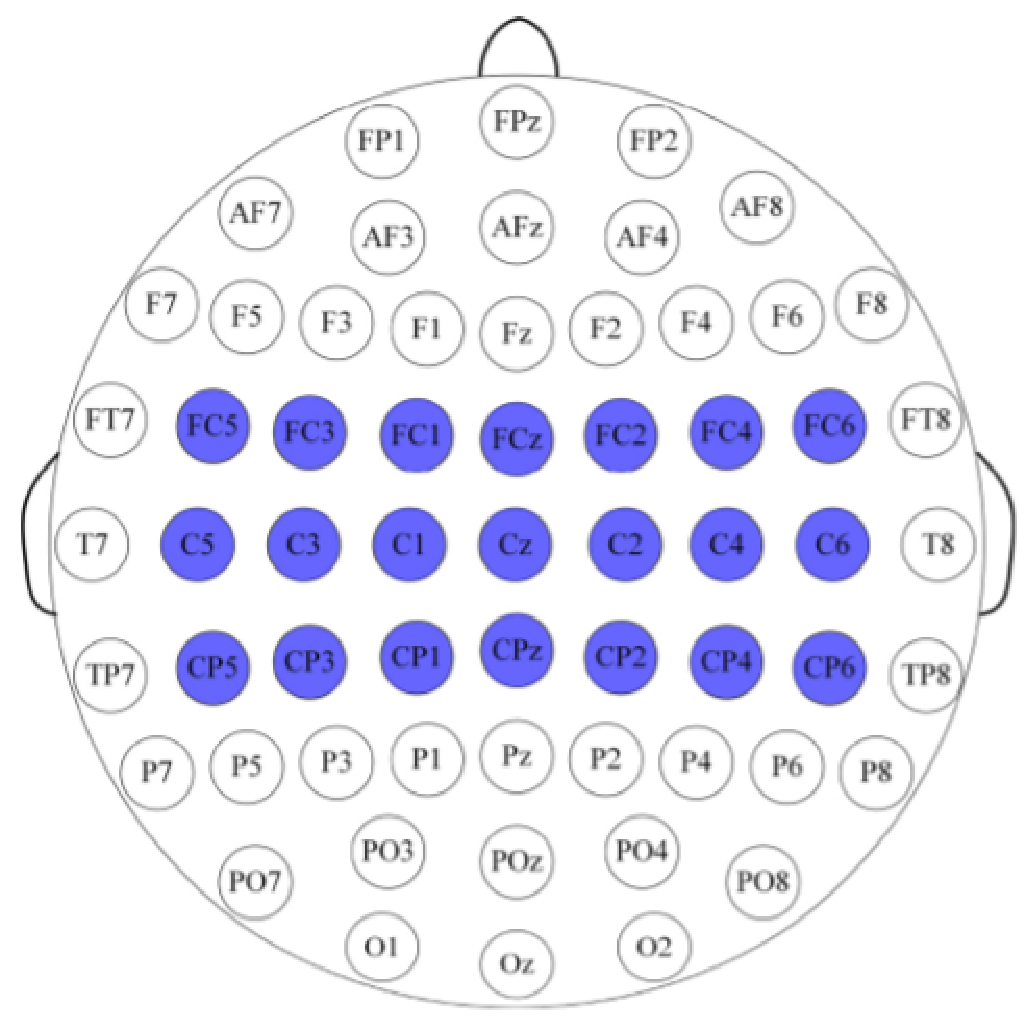
\includegraphics[width=\linewidth]{figures/fig2.eps}  % 插入图片,width 可以设置图片的宽度
  \caption{EEG electrodes placement according to the 10-20 system. The related motor imagery electrodes are identified in blue color.}  % 图片标题
  \label{fig:10-20}  % 给图片设置标签,方便引用
\end{figure}

EEG captures physiological activities of the body by recording electrical signals which are the produced postsynaptic potentials by cortical neurons \cite{sazgar2019overview}. The electrical signals are recorded via conducting electrodes that are placed on the scalp according to the well-known 10-20 international placement system as stated in Fig.~\ref{fig:10-20}, motor imagery related electrodes are identified in blue color \cite{Kwon2020}. Each electrode records a one-dimensional vector of raw EEG data. The signals are obtained on the three-dimensional scalp surface through volume conduction across multiple brain tissue \cite{sazgar2019overview}. Hence, EEG signals are prone to artifacts originating from different parts of the body like the eye, head, neck, or any other muscle. Moreover, the power cable of the recording device and electrode displacement might both cause some artifacts. This form of recording EEG produces weak, non-stationary, and low signal-to-noise ratio signals. Consequently, it complicates the classification and interpretation of signals belonging to a particular case of consideration.

Despite the inherent drawbacks in raw EEG, it has some advantages over other neurological imaging techniques. It characterized by low cost, portability, and causes no side effects because of its non-invasive style \cite{qiao2019deep}. Thus, EEG has a variety of applications whether as a screening method or for hypothesis-based diagnostics. Depending on the shape of waves, e.g. rapid spikes waves or slow waves, several forms of brain disorders can be assessed, such as epilepsy \cite{mardini2020enhanced}, tumors \cite{mardini2020enhanced}, Alzheimer \cite{pandya2020buildout}, sleep disorder \cite{geng2020novel}, etc.

Basically, the amplitude and frequency values in EEG signals are used for discriminating various physiological activities. The amplitude is normally fluctuating in microvolts. The frequency range in EEG signals can be split into several bands as shown in Table 1 \cite{wang2018lstm}. The most popular motor imagery frequency bands are also stated in the table. It should be noted that when the Alpha band is recorded from the sensorimotor cortex then it is called mu band. The Gamma band can be recorded consistently using internal electrodes in order to better capture it as it is being weak at the scalp \cite{padfield2019eeg}. Slightly different frequency bands or ranges may be found in the literature.

EEG signals are complex in their nature and there exists acute dependency of signal quality on the mental state of the user. Studies proved that the classification accuracy of an intelligent system for a certain task was better at the beginning of the trial than the accuracy at the end of that trial \cite{padfield2019eeg}. Therefore, recording or selecting an EEG dataset is crucial for training, validating, and testing machine learning models.

\subsection{Acquisition Process}

\begin{enumerate}
\item \emph{Preparation}.
Ambient electrical noise can significantly interfere with EEG recordings. When setting up a laboratory, and periodically throughout the course of data collection, it is advisable to check noise levels using a handheld gauss meter sensitive to the electrical noise frequency range emitted by power lines, computers, and other electrical appliances. In China, this frequency range is typically 50 Hz, while in the USA, it can be 60 Hz.

Ensure that the laboratory environment is quiet and free from electromagnetic interference. One effective method for reducing the influence of electrical noise is to collect EEG data in an electrically shielded room or chamber. If such a facility is not available, and a gauss meter indicates the presence of electrical noise, relocating the offending equipment a short distance away from the electrodes and electrode wires can often mitigate the impact of noise on recordings.

When the study participant arrives at the lab, make them feel comfortable, explain the experiment in detail, and ensure they understand all aspects of it. Have the subject sign the consent form and adjust the stimulation setup to their comfort (e.g., chair height, screen distance, or sound levels) to minimize movement and muscle tension, thereby avoiding interference with the EEG signals.

\item \emph{Adjusting the Equipment}.
Select the correct cap size by measuring the participant's head circumference in centimeters (hat size) around the widest point on the head using a flexible tape measure. Cap sizes typically range from 52 to 60 cm in increments of 2 cm. Most labs have 54, 56, 58, and 60 cm sizes as part of a standard EEG setup. If the measurement falls between sizes, try the next larger size. The cap should fit snugly. Ensuring a proper fit is crucial, as a cap that is too large may reduce the quality of EEG recordings or make electrode preparation and impedance reduction more challenging. To check the fit, ask the participant to nod their head up and down and turn it side to side. If the cap shifts, it is too big, and a smaller size should be used. Additionally, when the cap is on the participant’s head, gently press down on one of the electrode adaptors towards the scalp. If the adaptor bounces back, there may be too much space between the adaptor and the scalp, indicating that a smaller cap size should be tried. Once the correct cap size is determined, remove the cap from the head and snap in the electrodes.

Plug the electrodes into the EEG amplifier at the appropriate locations. Consult the EEG acquisition software materials for instructions on how to designate channels. Depending on the setup and equipment, it may be necessary to label the channels on the amplifier (e.g., Ground, FP1, CZ, REOG, LEOG).

Before placing the cap on the participant's head, roughly measure the distance between the participant's nasion (bridge of the nose) and inion (bump on the lower base of the skull: to find the inion, place your hand in the middle of the neck and slide upwards) using your hands. The FPz electrode should be placed about 10\% of this distance above the nasion in the middle of the forehead. Place the front of the cap on the participant's forehead with FPz in this position, ask the participant to hold the cap in place, and then pull the cap over the head. Next, adjust the position of the CZ electrode so it lies halfway between the nasion and the inion.

Minimize the impedance of the electrical connection between the electrode and the scalp by applying abrasive electrolyte gel. Specifically, fill syringes with abrasive electrolyte gel, and then fill the electrodes with gel using those syringes (ensure the plastic tip of the syringe touches the scalp). Gently scrub the scalp through the electrode opening by twirling the cotton end of the cotton swab between your thumb and index finger.

\item \emph{Begin Data Collection}.
Open the EEG acquisition software and load the experiment file. Observe the resting activity of all the electrodes, and ensure there are no “bad” channels; that is, electrodes that produce flat line signals or show excessive activity while the participant is resting. If any bad channels are suspected, it may be necessary to apply more electrode gel and scrub to minimize impedance or replace the electrode. Instruct the participant to avoid blinking and tensing muscles in their forehead or jaw, as these actions can introduce noise into the EEG data.

Once all the electrode signals appear acceptable, begin recording and start the experiment file. If collecting data for an MI experiment or other design where the timing of stimulus presentation is crucial for signal processing, carefully observe the first few trials to ensure that the stimulus presentation software is sending “trigger” markers for stimulus presentation. If timing markers are not being sent, the data cannot be processed using stimulus presentation as a reference point, which is essential for MI designs.

\end{enumerate}

\section{Data Processing}
\subsection{Preprocessing of raw data}
Raw EEG signals usually contain plenty of undesirable background noise that requires elimination before beginning the real analysis. Also, sometimes it is desirable to enhance the raw EEG to better fit the requirements. For those reasons, one or more of the listed below preprocessing methods \cite{tayeb2019validating, tang2020motor, ludwig2017investigation, reddy2019electroencephalogram} might be applied.

\begin{itemize}
  \item Notch filtering to remove power line noise at 50 Hz or 60 Hz.
  \item High-pass filtering with a low cutoff frequency to remove baseline drift.
  \item Band-pass filtering to select the desirable band(s).
  \item Clipping the amplitude of EEG signals either by forcing it to be within a specific range or based on the mean and the standard deviation.
  \item Canceling several samples from the beginning and\or from the end of the signal to remove possible acute artifacts.
  \item Normalizing the data to zero mean and unit variance using z-score. This can speed up the convergence and avoid trapping by local minima.
  \item Downsampling the signal for speeding up the computation and reducing memory storage.
  \item Selection of specific electrodes based on the goal of the application.
  \item Interpolating of corrupted signals.
  \item Artifact rejection such as the electrooculogram (EOG) and the electromyogram (EMG) artifacts. This can be achieved in different ways such as a thresholding-based method or data-driven method like the Independent Component Analysis (ICA).
  \item Referencing using either an electrode (Cz and Fz are often employed as reference electrodes) or the average of signals from all electrodes. Common average referencing (CAR) and Laplacian are widely used spatial filters. Referencing helps to eliminate some of the background noise.
\end{itemize}

\section*{Acknowledgement}
This research was supported by the National Natural Science Foundation of China Grant 61873321.



\bibliographystyle{IEEEtran}\bibliography{drwubib}


\begin{IEEEbiography}[{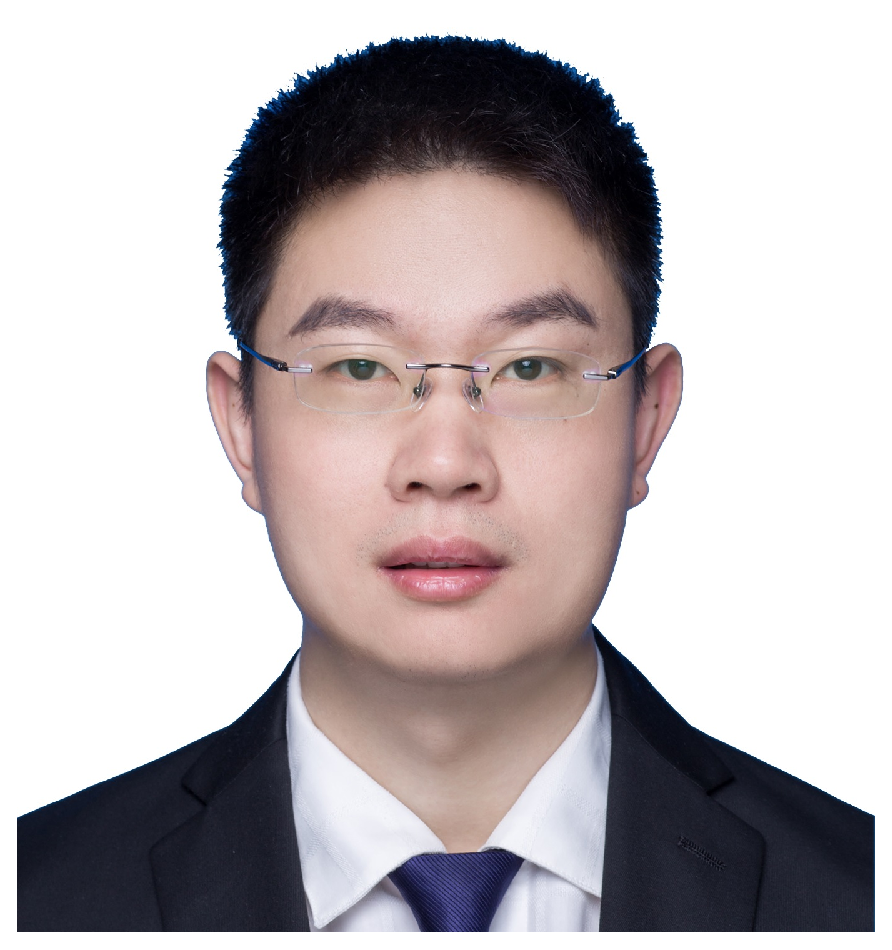
\includegraphics[height=1in,clip,keepaspectratio]{Wu}}]{Dongrui~Wu} (S'05-M'09-SM'14) received the BE degree in automatic control from the University of Science and Technology of China in 2003, the ME degree in electrical engineering from the National University of Singapore in 2005, and the PhD degree in electrical engineering from the University of Southern California in 2009. He is now Professor in the School of Artificial Intelligence and Automation, Huazhong University of Science and Technology, Wuhan, China, and Deputy Director of the Key Laboratory of Image Processing and Intelligent Control, Ministry of Education. His research interests include affective computing, brain-computer interface, computational intelligence, and machine learning. He has more than 110 publications, including a book entitled \emph{Perceptual Computing} (Wiley-IEEE Press, 2010).

Prof. Wu received the IEEE Computational Intelligence Society Outstanding PhD Dissertation Award in 2012, the IEEE TRANSACTIONS ON FUZZY SYSTEMS Outstanding Paper Award in 2014, the NAFIPS Early Career Award in 2014, the IEEE Systems, Man and Cybernetics (SMC) Society Early Career Award in 2017, and the IEEE SMC Society Best Associate Editor Award in 2018. He was also a finalist of another three Best Paper Awards. He was/is an Associate Editor of the IEEE TRANSACTIONS ON FUZZY SYSTEMS (2011-2018), the IEEE TRANSACTIONS ON HUMAN-MACHINE SYSTEMS (2014-), the IEEE COMPUTATIONAL INTELLIGENCE MAGAZINE (2017-), and the IEEE TRANSACTIONS ON NEURAL SYSTEMS AND REHABILITATION ENGINEERING (2019-).
\end{IEEEbiography}

\begin{IEEEbiography}[{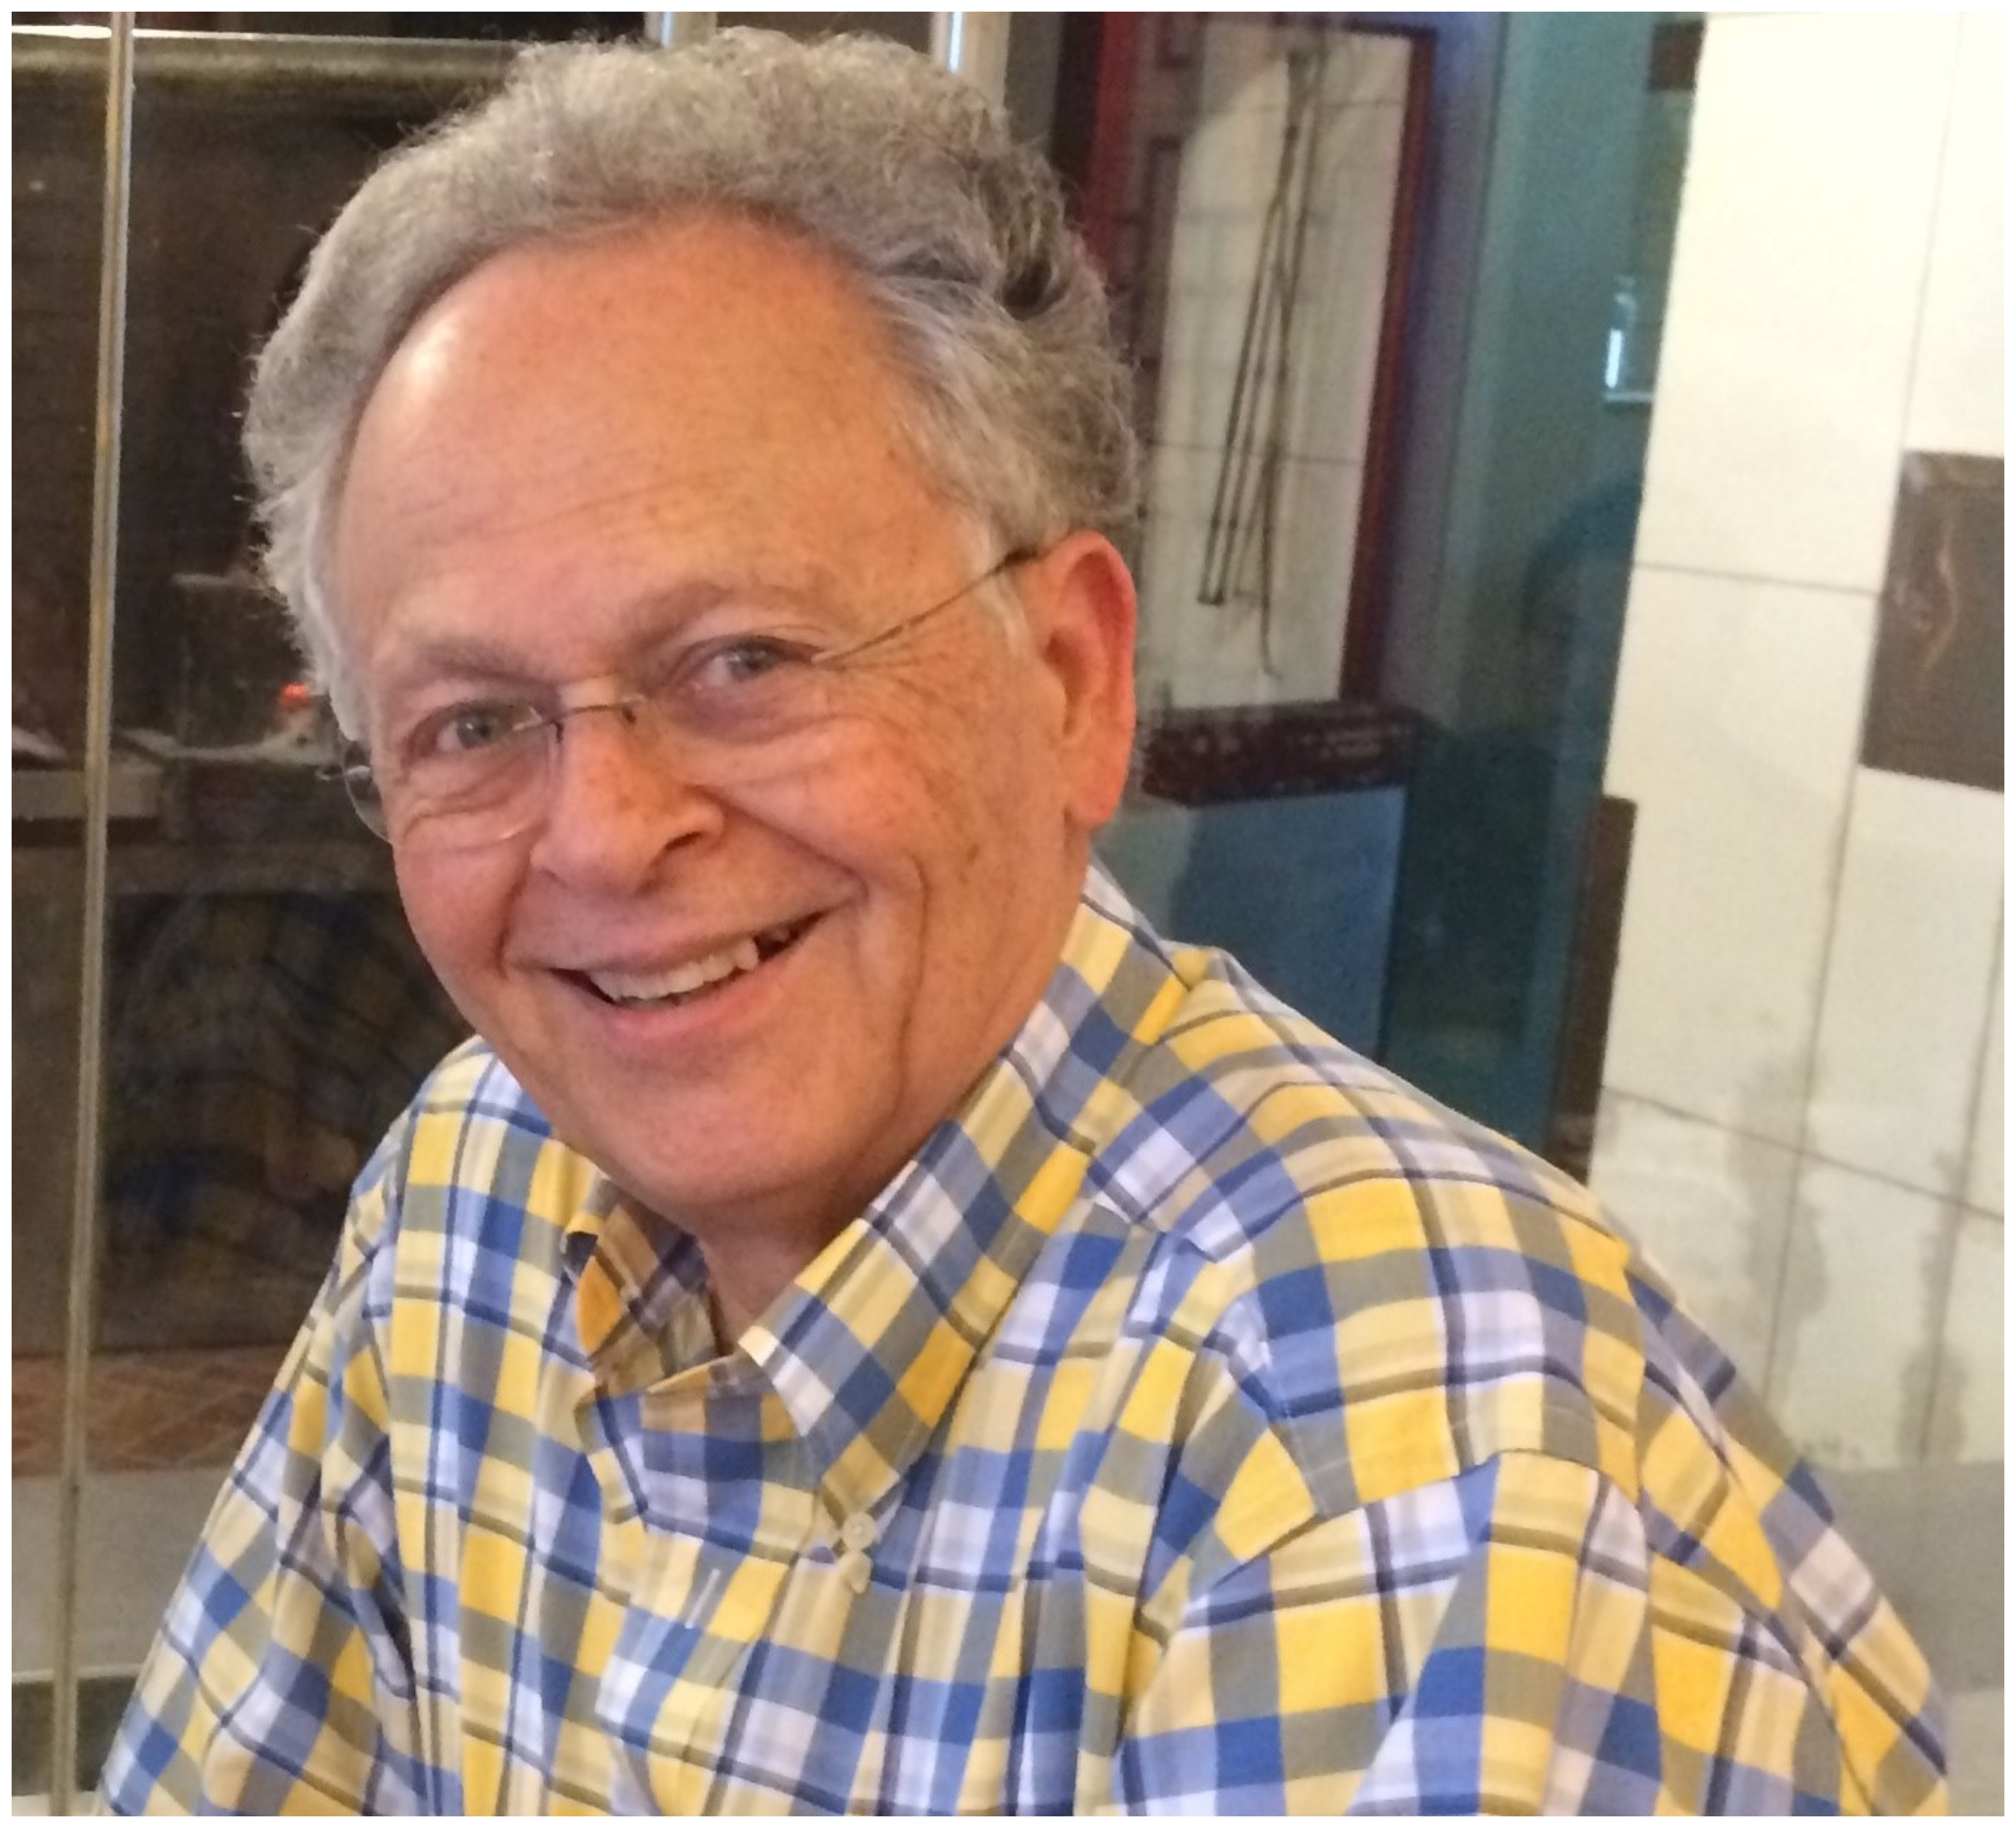
\includegraphics[width=1in,clip,keepaspectratio]{Mendel}}]{Jerry M. Mendel} (LF'04) received the Ph.D. degree in electrical engineering from the Polytechnic Institute of Brooklyn, Brooklyn, NY, in 1963. Currently, he is Emeritus Professor of Electrical Engineering at the University of Southern California in Los Angeles,  where he has been since 1974. He is also Tianjin 1000-Talents Foreign Experts Plan Endowment Professor and Honorary Dean of the College of Artificial Intelligence, Tianjin Normal University, Tianjin, China.

He has published over 570 technical papers and is author and/or co-author of 13 books, including Uncertain Rule-based Fuzzy Systems: Introduction and New Directions, 2nd ed. (Springer 2017), Perceptual Computing: Aiding People in Making Subjective Judgments (Wiley \& IEEE Press, 2010), and Introduction to Type-2 Fuzzy Logic Control: Theory and Application (Wiley \& IEEE Press, 2014). He is a Life Fellow of the IEEE, a Distinguished Member of the IEEE Control Systems Society, and a Fellow of the International Fuzzy Systems Association. He was President of the IEEE Control Systems Society in 1986, a member of the Administrative Committee of the IEEE Computational Intelligence Society for nine years, and Chairman of its Fuzzy Systems Technical Committee and the Computing With Words Task Force of that TC. Among his awards are the 1983 Best Transactions Paper Award of the IEEE Geoscience and Remote Sensing Society, the 1992 Signal Processing Society Paper Award, the 2002 and 2014 Transactions on Fuzzy Systems Outstanding Paper Awards, a 1984 IEEE Centennial Medal, an IEEE Third Millenium Medal, a Fuzzy Systems Pioneer Award (2008) from the IEEE Computational Intelligence Society for ``fundamental theoretical contributions and seminal results in fuzzy systems"; and, 2015 USC Viterbi School of Engineering Senior Research Award. His present research interests include: type-2 fuzzy logic systems and computing with words.
\end{IEEEbiography}

\end{document}
